\documentclass{article}
\usepackage[utf8]{inputenc}
\usepackage{amsmath}
\usepackage{natbib}
\usepackage{parskip}
\usepackage{tikz}
\bibliographystyle{jasa}
\usetikzlibrary{positioning,calc,backgrounds}


\title{Notater til masteren}
\author{johaskog }
\date{January 2021}

\parskip 0.2in %making spacing between paragraphs
\newcommand{\dd}{\mathrm{d}}





\begin{document}

\maketitle
%need this to plot the tikz trees. 
%This is needed for the tikzpicture:
\newcommand{\DoNode}[8][]{% (keys), name, loss1, loss2, loss3, CircleColour1, CircleColour2, radius
    %\pgfmathtruncatemacro{\tmpa}{round(360*#3/(#3+#4+#5))}
    %\pgfmathtruncatemacro{\tmpb}{round(360*(#3+#4)/(#3+#4+#5))}
    %\pgfmathtruncatemacro{\tmpa}{round(360*(#3/(#3+#4+#5)))}
    %\pgfmathtruncatemacro{\tmpb}{round(360*((#3+#4)/(#3+#4+#5)))}
    \pgfmathtruncatemacro{\tmpa}{round(360*(#3/(#3+#4+#5)))+90}
    \pgfmathtruncatemacro{\tmpb}{round(360*((#3+#4)/(#3+#4+#5)))+90}
    
    %\node[treenodeT, #1] (#2) {Loss0: #3 \\ Loss1: #4 \\ Loss2: #5};
    \node[treenodeT, #1, minimum size=2*#8cm] (#2) {};
    % and after that...
    \begin{scope}[on background layer]
        %\fill [blue!40] let \p1 = ($(#2.0)-(#2.center)$) in
        %    (#2.center) -- (#2.0) arc(0:\tmpa:{veclen(\x1,\y1)}) -- cycle;
        %\fill [red!40] let \p1 = ($(#2.0)-(#2.center)$) in
        %    (#2.center) -- (#2.\tmpa) arc(\tmpa:\tmpb:{veclen(\x1,\y1)}) -- cycle;
        %\fill [green!30] let \p1 = ($(#2.0)-(#2.center)$) in
        %    (#2.center) -- (#2.\tmpb) arc(\tmpb:360:{veclen(\x1,\y1)}) -- cycle;
        \fill [blue!30] let \p1 = ($(#2.0)-(#2.center)$) in
            (#2.center) -- (#2.0) arc(0:\tmpa:{veclen(\x1,\y1)}) -- cycle;
        \fill [red!30] let \p1 = ($(#2.0)-(#2.center)$) in
            (#2.center) -- (#2.\tmpa) arc(\tmpa:\tmpb:{veclen(\x1,\y1)}) -- cycle;
        \fill [green!30] let \p1 = ($(#2.0)-(#2.center)$) in
            (#2.center) -- (#2.\tmpb) arc(\tmpb:450:{veclen(\x1,\y1)}) -- cycle;
%        \draw [#6!20] let \p1 = ($(#2.0)-(#2.center)$) in
%            (#2.center) -- (#2.\tmpb) arc(\tmpb:360:{veclen(\x1,\y1)}) -- cycle;
%        \draw[color = #6] (#2.center) circle (1.5cm);
        \draw[color= #6, very thick] (#2.center)+(0,#8cm) arc (90:270:#8cm);
        \draw[color = #7, very thick] (#2.center)+(0,-#8cm) arc (270:360:#8cm);
        \draw[color = #7, very thick] (#2.center)+(#8cm,0) arc (0:90:#8cm);
    
    \end{scope}
}


\newpage
%\section{Introduction}
\chapter{Introduction}
Schizophrenia is a psychotic disorder where at least two of the symptoms delusions, hallucinations, disorganized speech, grossly disorganized or catatonic behaviour or negative symptoms such as reduced emotional expressions and lowered motivation, have to be present. 
Delusions are beliefs that will not change if contradicting evidence is presented. The most common type of delusions are persecutory delusions. People that have those kinds of delusions might think that they will be hurt, injured, tormented or so on by others. Referential delusions are also common. Then one are putting meaning into comments, gestures and actions, thinking that they are about oneself, when they not necessarily are. Completely improbable beliefs are called bizarre delusions. These are delusions others find far-fetched, and they are things that cannot happen in real life. A bizarre delusion could for example be that a person believes that their organs have been removed replaced by someone else's organs without there being any scars or other evidence of that happening. A delusion that is not bizarre could be that you think you are under police surveillance without there being any evidence of that. It might be hard to distinguish between delusions and strongly held ideas. The main distinction is about the degree of conviction, and how much or little the beliefs can be amended when contradicting facts are presented \citep{dsm-5}. 
%Hallucinations are sensory impressions that happen without any external stimulus. Hence, others usually does not experience the same impressions. The hallucinations are perceived as normal experiences to the person having them. For schizophrenic people, they often occur as voices which can be distinguished from the persons own thoughts. 
%Disorganized speech means that one are switching between topics rapidly and giving unrelated answers to questions. 
%Grossly disorganized behavior is also referred to as abnormal behavior, and catatonic behavior means that one has a dampened reaction to things happening around oneself. (All of the above is from DSM-5).


Delusions are one of the main characteristics of schizophrenia as it appears in about three out of four of those diagnosed \citep{garety2011}. Researchers have been trying to understand how the delusions are formed and maintained in order to improve treatment \citep{dudley_meta_2016}. One important finding is that deluded individuals seem to make decisions based on less evidence than both healthy and psychiatric controls. This is often referred to as a "jumping to conclusions" (JTC) bias \citep{dudley_meta_2016}. A person with this bias might reach decisions or form beliefs before reaching realistic conclusions, and thus accept unrealistic ideas. They are therefore more prone to delusions \citep{dudley_meta_2016}. The hope is that if we can detect the JTC bias, we can reduce the delusional thinking, and thus prevent delusions \citep{dudley_meta_2016}.

The JTC bias is traditionally tested with a probabilistic reasoning task called the beads task. The participants are presented with two jars containing beads of two colours, for example red and blue. The two jars have opposite ratios of each colour, meaning that if the first have 85\% red beads and 15\% blue, the second has 15\% red and 85\% blue beads. The participants are told that beads are drawn from one of the jars, and their task is to find out which one that is. They are told to choose only when they are completely sure, and they draw as many beads as they want. The beads are drawn sequentially, and after each draw the participants are asked if they want to choose which jar beads are drawn from or if they want to draw more beads. One are usually said to have a JTC bias if one decides after one or two beads \citep{moritz2017}. However, the beads task has shown to pose some problems.

Some of the first to use the beads task were \citet{huq1988}. Already in that article they presented some of the problems with the beads task. They used an 85-15 ratio of the beads. When the two first beads that are drawn are of the same colour, it is a 97\% probability that the beads are from the jar with 85\% of the beads in that colour. One might therefore argue that choosing jar at that point is reasonable, and that it does not show a JTC bias. Deluded individuals make decisions earlier that the control groups, but \citeauthor{huq1988} argue that non-deluded individuals are more conservative, and that people with delusions simply cancel out that bias when gathering less information. In an article by \citet{moritz2017}, other problems with the beads task are discussed. For example that many participants seem not to understand that all the beads are drawn form the same jar. This makes them think that after each bead is drawn, they have to guess which jar that bead is drawn from. These participants are then classified to have a JTC bias. We can also see that it is common to make logical errors due to miscomprehension. In an article by \citet{moritz2005}, they found that 52\% of the schizophrenic participants and 23\% of the healthy controls had at least one response that was not logical. The participants that misunderstand are more likely to choose early. \citet{moritz2017} further states that the beads task is correlated with intelligence. Lack of intelligence might be a reason for or a confound for misunderstanding the task. It is also stated that confidence influences decision-making. The participants are asked to choose when they are completely sure which jar the beads are drawn from, which could make more confident participants decide earlier. We might also conclude that hasty decisions are made because the participants like to take risks or that they are not cautious, or both. However, other tasks that accounts for confidence also display a JTC bias with the delusion-prone participants. Additionally, there is only a one-dimensional sequence of events in the beads task. Thus, it is harder to find different versions to test multiple times. 

The box task has been suggested as an alternative to the beads task. Here, the participants are presented with a grid of a fixed number of boxes. When a box is opened, one out of two colours is displayed, for example blue and red. The participants are told that one of the colours are always in majority, and their task is to find out which one \citep{moritz2017}. They can open as many boxes as they want before they make a decisions. Both the number of boxes and the ratio of the two colours can be changed for each new trial. 

In this report we model how the participants make decisions in the box task. In the version of the box task used here, there are twelve boxes. We use two different versions of the box task. The first one is an unlimited one, where the participants can open as many boxes as they want, even until all twelve boxes are opened, before reaching a decision. In the second version, the participants are told that the test will terminate at a random point. If the test terminates before the participant has decided what the majority colour is, this counts as a failed trial. We call this the limited version. In Figure \ref{picture_of_box_task}, we see a limited trial of the box task with red and blue boxes. The participant have opened two boxes, and has to choose whether to open another box or to choose that either blue is the dominant colour, or that red is. 

\begin{figure}
    \centering
    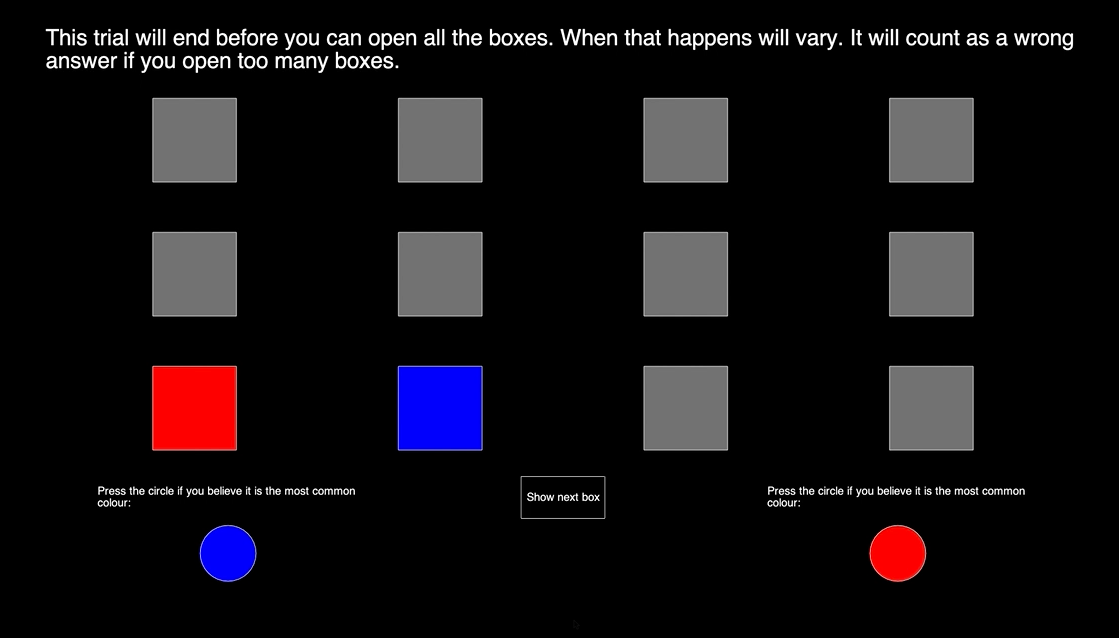
\includegraphics[scale=0.486]{Sections/Box task 2.png}
    \caption{Describe the figure}
    \label{picture_of_box_task}
\end{figure}

We have data from 76 participants that have done 10 trials each of the box task. The first trial was a practice trial of the limited version followed by three unlimited and six limited trials. We can model the decisions the participants make using a Softmax model, and fit this model to each participant with maximum likelihood estimation. Thus, we find the maximum likelihood estimates in the Softmax mode. Then, we find confidence intervals for each of these estimates using parametric bootstrapping and percentile intervals. 

As an input in the Softmax model we have an Ideal observer solution of the box task. An Ideal observer is a participant that always make optimal, or ideal, choices, and thus finds the best solution \citep{idealObs}. Each time a box is opened, the participant have three options. The first is to choose that blue is the majority colour, the second that red is, and the third option is to open another box. For each of these alternatives we have found loss functions, which represent the cost of choosing the different options. An Ideal Observer would always choose the alternative with the least loss, and would end up with the overall optimal or ideal solution. In this report we are assuming that the total number of red boxes is binomial distributed with parameters 12 and $\theta$. Each time a box is opened, the probability that the box is red is $\theta$ and $1-\theta$ that the box is blue. We also assume a beta prior for $\theta$ with parameters $\gamma$ and $\kappa$. If we have any prior beliefs about the probability of the different colours, this knowledge can be incorporated here. If both $\gamma$ and $\kappa$ is one, this is a uniform prior, meaning that $\theta$ has the same probability of being each possible value between zero and one. 



%(something about: here they are not said to answer when they are completely sure? compared to the beads task, where they are said to answer when comp sure. Jeg klarer ikke å finne ut hvor det står??)





%In this report we are firstly going to find an Ideal Observer solution of the box task. We assume that each time a box is opened, the probability that this box is red is $\theta$, and then that the probability that it is blue is $1-\theta$. We also choose a prior distribution for $\theta$, a beta distribution with parameters $\gamma$ and $\kappa$. If we have any prior beliefs about the probability of the different colours, this knowledge can be incorporated here. 
%Each time a box is opened, the participant have three options. The first is to choose that blue is the majority colour, the second that red is, and the third option is to open another box. For each of these alternatives we have found loss functions, which represent the cost of choosing the different options. An Ideal Observer would always choose the alternative with the least loss, and would end up with the overall best(?) solution. (should i say something about the fact that i have found another ideal observer solution assuming other things in the specialization thesis?)


% - We want to model how participants make decisions in the box task. We have data from 76 participants who have done 10 different trials of the box task, one practice trial that was limited, then followed by 3 unlimited and 6 limited trials. 
% - we can model this using a softmax model, and an Ideal Observer solution of the box task. From the specialization thesis we already have an Ideal observer solution assuming that the number of red boxes is uniformly distributed. 
% - three options each time a box is opened, loss functions for each option. An ideal observer always chooses the choice with the least loss. If we always do the best choice, we end up with the best solution.
%  - in this report we will also find another Ideal observer solution assuming a binomial distribution of the number of red boxes, and a beta prior for $\theta$. If we have beta(1,1), this will be a uniform prior. 

-paragraph about how this report is structured. 
\newpage
\chapter{Background Theory}
%\section{Theory}
In this chapter, we go through some of the statistical theory used in this report. This includes the theorem of total probability, Bayes' theorem, the beta and gamma functions, Bayesian modelling, loss functions, the law of total expectation, the softmax function, maximum likelihood estimation and bootstrapping.  

\section{The Theorem of Total Probability}
The theorem of total probability is often used when we want to find some probability, and this probability is hard to find. Then, sometimes it might be easier to find that probability if we condition on something, and use the theorem of total probability. 
\begin{theorem}[Theorem of Total Probability, Continuous Variables]
If we have a continuous variable, $\Theta$, and a discrete variable, $U$, and both $P(U=u|\Theta=\theta)$ and  $f_\Theta(\theta)$ are known for all $\theta$, then we can find $P(U=u)$ from \citep{schay2016introduction} 
\begin{equation}
    \label{lawoftotprob}
    P(U=u) = \int_{-\infty}^{\infty} P(U=u|\Theta=\theta)f_{\Theta}(\Theta=\theta) \: \dd \theta.
\end{equation}
\end{theorem}

\begin{comment}
In \citet{schay2016introduction}, the theorem of total probability for continuous variables is stated as 
\begin{theorem}[Theorem of Total Probability, Continuous Versions]
 For a continuous random variable Y and any event A, if $f_{Y|A}$ and $f_Y$ exists for all y, then
\begin{equation}
   % \label{lawoftotprob}
    P(A) = \int_{-\infty}^{\infty}
    P(A|Y=y)f_Y(y) dy.
\end{equation}
\end{theorem}
\end{comment}




Consider, for example, two discrete random variables $U$ and $V$ that are conditionally independent given the continuous stochastic variable $\Theta$. To find the probability that $U+V$ is equal to some integer $j$, we can use the theorem of total probability to condition on theta. Thus,
\begin{equation*}
    P(U+V=j) = \int_{-\infty}^\infty P(U+V=j|\Theta=\theta)f_{\Theta}(\Theta=\theta) \: d\theta.
\end{equation*}
Later, we can exploit the conditional independence. If $\theta$ is a probability defined on the interval (0,1), this will be integrated on that interval, such that 
\begin{equation*}
    P(U+V=j) = \int_{0}^1 P(U+V=j|\Theta=\theta)f_{\Theta}(\Theta=\theta) \: d\theta.
\end{equation*}
%Mer utfyllende her?




\section{Bayes' Rule}
We can use Bayes' rule to find conditional probabilities and distributions. 
\begin{theorem}[Bayes' Rule]
Consider two events, $A$ and $B$. We can find the probability of $A$ given event $B$ by the use of the probability of event $B$ given $A$ and the probabilities of the events $A$ and $B$ separately \citep{statinf}. Hence,
\begin{equation}
\label{bayesrule}
    P(A|B)=\frac{P(B|A)P(A)}{P(B)}.
\end{equation}
\end{theorem}


As an example, consider a discrete random variable, $U$. We can find the probability that $U$ is greater than or equal to 7, and condition on it being different from six by using \eqref{bayesrule}. Then $U \geq 7$ is an event, and $U\neq6$ is another event. Thus,
\begin{equation}
    P(U\geq 7|U\neq6) = \frac{P(U\neq6|U\geq7)P(U\geq7)}{P(U\neq6)}.
\end{equation}



\section{The Beta and Gamma Functions}
Later, we will use the beta and gamma functions and some of their properties. These are therefore stated here. This theory can for example be found in \citet{statinf}. The gamma function for a parameter $\kappa$ is 
\begin{equation*}
    \label{gamma_func}
    \Gamma(\kappa) = \int_0^\infty t^{\kappa-1}e^{-t} \dd t.
\end{equation*}
A useful property of the gamma function is that it is recursive. Hence,
\begin{equation}
\label{gamma_recursive_property}
    \Gamma(\kappa+1) = \kappa \Gamma(\kappa), \quad \kappa>0 .
\end{equation}

Additionally, the beta function with parameters $\gamma$ and $\kappa$ is defined as
\begin{equation}
\label{beta_function}
    \mathrm{B}(\gamma,\kappa) = \int_0^1 \theta^{\gamma-1}(1-\theta)^{\kappa-1} \: \dd \theta.
\end{equation}
We can express the beta function as a product of gamma functions. This yields
\begin{equation}
\label{beta_as_gamma}
    \mathrm{B}(\gamma,\kappa) = \frac{\Gamma(\gamma)\Gamma(\kappa)}{\Gamma(\gamma+\kappa)}.
\end{equation}



\section{Bayesian Modelling}
\label{theory_bayesian_modelling}
Consider a stochastic variable, $U$, that has a probability density function $f(u|\theta)$, where $\theta$ is a parameter upon which $U$ depends. In classical statistics, $\theta$ is said to be a fixed but unknown value. The goal is to find this one true value. 
However, in Bayesian statistics we consider $\theta$ as a stochastic variable, such that $\theta$ has a density function. 
Here, the goal is to find the underlying density. To do so we propose a prior distribution for $\theta$, $f(\theta)$. The prior distribution represents the prior knowledge we have about $\theta$ before observing any data. That could be our own subjective believes about the parameter or information based on other previously collected data or studies. One could also choose a prior distribution that does not say anything about the parameter at all. This is called a non-informative prior, and it is often used when we have none or little prior information about the parameter \citep{givens2012computational}. 
If we have collected data, denoted $u$, we can update our prior beliefs with the information we get from that data. The resulting distribution is called the posterior distribution of $\theta$, $f(\theta|u)$. We can find this using Bayes' theorem, and it includes both the prior information we have and the new information we get from the data. 

Consider a discrete stochastic variable, $U$, that has a sampling distribution $P(U=u|\theta)$, and let $P(U=u)$ be the marginal distribution of $U$. Additionally, let $f(\theta)$ be the prior distribution of $\theta$. Using Bayes' rule as it is stated in \eqref{bayesrule}, we get that the posterior distribution of $\theta$ given $u$, $f(\theta|u)$, can be expressed as \citep{statinf}
\begin{equation*}
    f(\theta|u) = \frac{P(U=u|\theta)f(\theta)}{P(U=u)}.
\end{equation*}
We can sometimes exploit the fact that the posterior distribution is proportional to the numerator in the above expression. This is because the denominator is a normalising constant. Hence,
\begin{equation}
    \label{posterior_proportional}
    f(\theta|u) \propto P(U=u|\theta)f(\theta).
\end{equation}
If \eqref{posterior_proportional} has the form of a known distribution, then that known distribution is the posterior distribution. 

As an example, consider a random variable, $U$, that is binomially distributed with parameters 12 and some probability, $\theta$. Thus,
\begin{equation*}
    \left( U|\Theta=\theta \right) \sim \mathrm{Binomial}(12,\theta).
\end{equation*}
Hence, the probability that we have $u$ successes out of twelve, given $\theta$, is
\begin{equation}
\label{binomial_12_ex}
    f(u|\theta) = \binom{12}{u} \theta^{u} (1-\theta)^{12-u}.
\end{equation}
As $\theta$ is a probability, its value is on the interval $[0,1]$. We know that the beta distribution is conjugate with the binomial distribution and has value between 0 and 1 \citep{statinf}, thus we choose a beta prior for $\theta$ with parameters $\gamma$ and $\kappa$. Hence,
\begin{equation}
\label{theta_with_beta_prior}
    \Theta \sim \mathrm{Beta}(\gamma,\kappa). 
\end{equation}
The prior density of $\Theta$ is then
\begin{equation}
    \label{betadistribution}
    f(\theta) = \frac{1}{\mathrm{B}(\gamma,\kappa)}\theta^{\gamma-1}(1-\theta)^{\kappa-1},
\end{equation}
where $B(\gamma,\kappa)$ is the beta function as defined in \eqref{beta_function}.
We can find the posterior distribution of $\theta$ using \eqref{posterior_proportional}, \eqref{binomial_12_ex} and \eqref{betadistribution}. Thus,
\begin{equation*}
    \begin{aligned}
        f(\theta|u) 
        &\propto f(u|\theta)f(\theta)\\[6pt]
        &\propto \binom{12}{u} \theta^{u} (1-\theta)^{12-u} \frac{1}{\mathrm{B}(\gamma,\kappa)}\theta^{\gamma-1}(1-\theta)^{\kappa-1}
    \end{aligned}
\end{equation*}
All the factors that do not include $\theta$ are constants, and we collect them together as one constant, denoted $C$. Then
\begin{equation*}
    \begin{aligned}
        f(\theta|u) 
        \propto C \: \theta^{u+\gamma-1}(1-\theta)^{12-u+\kappa-1}.
    \end{aligned}
\end{equation*}
We can see that this is proportional to a beta distribution like the one in \eqref{betadistribution}, but in this case with parameters $u+\gamma$ and $12-u+\kappa$. Hence, the posterior distribution is a beta distribution with these parameters, 
\begin{equation*}
    \Theta|U=u \sim \mathrm{Beta}(u+\gamma,12-u+\kappa).
\end{equation*}






\section{Loss Functions}
\label{theory_loss_functions}
A loss function typically says something about the cost, or loss, of an action related to a parameter. Let $\Omega_{\delta}$ be the action space, consisting of all the actions that we can do, where $\delta$ is an action. Then,
\begin{equation*}
    \delta \in \Omega_{\delta}.
\end{equation*}
Additionally, let $z$ be the true, but unknown state of nature, where 
\begin{equation*}
    z \in \Omega_z.
\end{equation*} 
We can define a loss function that depends on $z$ and $\delta$, which we denote $L(z,\delta)$. This is then the loss when making a decision, $\delta$, regarding $z$ \citep{statisticalDecisionTheoryLiese2008}.

A loss function could for example be the 0-1-loss function. If for example $\Omega_{\delta}= \Omega_z = \{0,1\}$, the loss function could be
\begin{equation}
\label{loss_func_indicator}
    L(z,\delta) = I(z \neq \delta),
\end{equation}
where $I$ is an indicator function such that
\begin{equation*}
    L(z,\delta) =
    \begin{cases}
        0,&  \text{if } z = \delta, \\
        1,&  \text{if } z \neq \delta.
    \end{cases}
\end{equation*}

In some cases, we would like to find the expected value of the loss function. Taking the expected value of an indicator function gives the probability that the event is happening \citep{algdat}. Hence, taking the expectation of \eqref{loss_func_indicator} gives
\begin{equation}
\label{expectation_of_loss_func_general}
    E[L(z,\delta)] = E[I(z\neq\delta)] = P(z\neq\delta).
\end{equation}



As an example, consider the box task with twelve boxes that could be either blue or red once they are opened. We define a stochastic variable, $X_i$, that represents the colour of the $i$-th opened box, such that 
\begin{equation}
\label{def_of_Xi}
    X_i =
    \begin{cases}
        0,& \text{if box }i \text{ is blue,}\\
        1,& \text{if box }i \text{ is red.}
    \end{cases}
\end{equation}
When $i$ boxes are opened, let $X_{1:i}$ denote the colours of the $i$ boxes, such that
\begin{equation}
\label{def_of_X1:i}
    X_{1:i} = (X_1,X_2,...,X_{i}).
\end{equation}
Additionally, let $Z$ be the colour that is in the majority when all twelve boxes are opened, the true majority colour. This is also a stochastic variable as it depends on the colours of the twelve boxes, the $X_i$'s. We define $Z$ as
\begin{equation}
\label{def_of_Z}
    Z = I\left(\sum_{j=1}^{12}X_j > 6\right).
\end{equation}
Then,
\begin{equation}
\label{Z_true_majority}
    Z = 
    \begin{cases}
        0,& \text{if blue is the true majority colour,} \\
        1,& \text{if red is the true majority colour.}
    \end{cases}
\end{equation}
Also, let $\delta$ be the choice the participant makes about which colour that is the dominant colour, such that
\begin{equation*}
    \delta = 
    \begin{cases}
        0,& \text{if the participant chooses blue as the majority colour,}\\
        1,& \text{if the participant chooses red as the majority colour}.
    \end{cases}
\end{equation*}
We can then define a loss function for the choice that the participant makes. This can be a 0-1 loss as in \eqref{loss_func_indicator}, and the loss function can therefore be defined as 
\begin{equation}
\label{loss_func_example}
    L(Z,\delta) = I(Z \neq \delta),
\end{equation}
Then, the loss is zero if the participant chooses the right colour as the majority colour and one if she chooses the wrong colour. 

To find the expected loss, we take the expectation of the loss function. As $Z$ depends on the colours of the twelve boxes, we condition on the colour of the already opened boxes, $ X_{1:i}=x_{1:i}$. The expectation of the loss function is then
\begin{equation*}
    E[L(Z,\delta)|X_{1:i}=x_{1:i}] = E[I(Z\neq \delta)|X_{1:i}=x_{1:i}].
\end{equation*}
As in \eqref{expectation_of_loss_func_general}, this expectation is the probability that $\delta \neq Z$, but here the probability depends on $X$. Thus,
\begin{equation}
\label{exp_loss_theory}
    E[L(Z,\delta)|X_{1:i}=x_{1:i}] = P(Z\neq \delta|X_{1:i}=x_{1:i}).
\end{equation}



%(Not sure if I should include this as this was fine when the loss func was if red or blue was teh right color, but now I have 3 decisions, and not two, and then teh 0-1-loss does not count, but it counts if we only talk about the two first decisions, decision 0 and 1.)





\section{The Law of Total Expectation}
Let $\{A_1,A_2,...,A_k\}$ be a partition of the sample space, $S$. Thus, there are $k$ non-overlapping parts, such that $A_i \cap A_j = \emptyset$, $\forall \:
i \neq j$. Then we also have that $S = A_1 \cup A_2 \cup...\cup A_k$. If we want to find the expectation of an event, $B$, and we have the expectation of $B$ on each of these partitions, we can use the law of total expectation. It states that
\begin{equation}
    E[B] = \sum_i E[B|A_i]P(A_i).
\end{equation}
This can also be used to find the expectation of functions \citep{schay2016introduction}. Let $g(B)$ be the function that we want to take the expectation of, then
\begin{equation}
\label{law_tot_exp_func}
    E[g(B)] = \sum_i E[g(B)|A_i]P(A_i).
\end{equation}

Later we will use the law of total expectation when we find the expectation of a loss function that says something about the loss of opening the next box in the box task. This expected loss is dependent on the colour of the box that will be opened. Thus, to find that expected loss, we use the law of total expectation and condition on the colour of the following box. 

%Again consider the box task. Let $\delta_i=2$ denote the choice of opening another box when $i$ boxes already are opened. We can in addition to the loss functions found above, \eqref{loss_func_example}, find a loss function for the choice of opening the next box. This loss function is dependent on the choice that are made after the next box is opened as well. We denote these as $\delta_{(i+1):12}$, and thus, we denote this loss function as $L(Z,\delta_i=2,\delta_{(i+1):12})$ (senere kaller jeg disse videre valgene for $IO(\textbf{x}_{i},0)$, men det blir litt mange greier å ta med her. hva skal jeg gjøre md det?). 

%The expectation of this loss function is dependent on the colour of the next box, $X_{i+1}$. We do not know the colour of that box, but we can find probabilities for the box being blue and red given the colour of the first $i$ boxes, $P(X_{i+1}=0|\textbf{x}_i)$ and $P(X_{i+1}=1|\textbf{x}_i)$, respectively. We can then find the expectation of this loss function using \eqref{law_tot_exp_func}, and condition on $X_{i+1}$. Then, 
%\begin{equation*}
%    E[L(Z,\delta_i=2,\delta_{(i+1):12})|\textbf{x}_i] = \sum_{j=0}^1
%    E[L[Z,\delta_{(i+1):12}|\textbf{x}_i]P(X_{i+1}=j|\textbf{x}_i).
%\end{equation*}
%Er dette litt mye greier å ta med her? Feks mtp notasjonen. Og er notasjonen godt nok forklart her?






\section{The Softmax Function} \label{section_theory_softmax}
The softmax function is commonly used in classification problems with more that two classes \citep{softmax}. Consider a decision, $\Delta$, which now is a stochastic variable for which we want to construct a distribution. We find a probability mass function for $\Delta=\delta$ using a softmax function. Let there be $D$ decisions, such that
\begin{equation*}
    \delta \in \{0,1,2,...,D-1\}.
\end{equation*}
Additionally, let $\EE_{\delta}(\vp)$ be values tied to each decision that depends on some parameters, $\vp$. The probability mass function for each decision, $\delta$, could be found using a softmax function, such that
\begin{equation}
\label{softmax_in_theory}
    \begin{aligned}
        f(\delta|\vp,\eta) = \frac{\text{exp}(- \eta \EE_{\delta}(\vp))}{\sum_{d=0}^{D-1} \text{exp}(-\eta \EE_{d}(\vp))},
    \end{aligned}
\end{equation}
where $\eta$ is some parameter. 

These decisions could, for example, be the three choices we have each time we open a box in the box task. These choices are that blue is the majority colour, or that red is, denoted $\delta=0$ and $\delta=1$, respectively. The last choice is to open another box, which we denote $\delta=2$. Then, we let $\EE_0(\vp)$ be the expected loss when choosing that blue is the majority colour, similarly to \eqref{exp_loss_theory}. Additionally, we let $\EE_1(\vp)$ and $\EE_2(\vp)$ be the expected loss of choosing red as the majority colour and of opening another box, respectively. Then, the probability mass function for $\delta$ could be as in \eqref{softmax_in_theory}. We then have a probability mass function for each of the three decisions that depend on the expected losses, parameters $\vp$ and some parameter $\eta$.




\section{Maximum Likelihood Estimation}
\label{section_theory_mle}

Maximum likelihood estimation is used to find estimates for parameters in a distribution. These are the estimates that, as the name implies, maximises the likelihood, and for short, we call them MLEs. Assume that we have probability distribution for a stochastic variable, $\Delta$, and consider $n$ samples, $\delta_1,\delta_2,...,\delta_n$, of $\Delta$. Denote the probability mass function for each of these $\delta$'s as $f(\delta|\vp)$, where $\vp$ contains the parameters in the probability mass function. If the $\delta_i$'s are independent, the likelihood function is defined as
\begin{equation}
\label{likelihood}
    L(\vp|\delta_1,\delta_2,...,\delta_n) =  \prod_{i=1}^{n} f(\delta_i|\vp).
\end{equation} 
The MLEs are then the estimates of $\vp$ that maximises this function, and they are usually denoted $\hat{\vp}$. It is often hard to maximize the likelihood function, then it might be easier to take the logarithm of the likelihood function and maximize that instead. This is called the log likelihood function, and is normally denoted as $l$. Thus,
\begin{equation}
\label{chap2:log_likelihood}
    \begin{aligned}
        l(\vp|\delta_1,\delta_2,...,\delta_n) 
        =& \text{log}\left(L(\vp|\delta_1,\delta_2,...,\delta_n)\right)\\
        =& \text{log}\left(\prod_{i=1}^{n} f(\delta_i|\vp) \right).
    \end{aligned}
\end{equation}
As the logarithm of products is the sum of the logarithms, we get that the log likelihood is
\begin{equation}
\label{chap2:log_likelihood2}
    \begin{aligned}
        l(\vp|\delta_1,\delta_2,...,\delta_n) = \sum_{i=1}^n \text{log}(f(\delta_i|\vp)).
    \end{aligned}
\end{equation}
Maximizing this will give the same maximum point as if we maximize the likelihood function \citep{statinf}. 

As an example, consider that the $\delta_i$'s have probability mass function as in \eqref{softmax_in_theory}. The parameters that we want to find estimates for are then $\vp$ and $\eta$. If we have $n$ samples of $\Delta$, denoted $\delta_i$, where $i \in \{1,2,...,n\}$,
the likelihood function would be
\begin{equation*}
    \begin{aligned}
        L(\vp,\eta|\delta_1,\delta_2,...,\delta_n) 
        =& \prod_{i=1}^{n} f(\delta_i|\vp,\eta)\\[6pt]
        =& \prod_{i=1}^{n}
        \frac{\text{exp}(- \eta \EE_{\delta_i}(\vp))}{\sum_{d=0}^{2} \text{exp}(-\eta \EE_{d}(\vp))}.
    \end{aligned}
\end{equation*}
The log likelihood would then be
\begin{equation*}
    \begin{aligned}
        l(\vp,\eta|\delta_1,\delta_2,...,\delta_n) =& \sum_{i=0}^N \text{log}\left( \frac{\text{exp}({-\eta \EE_{\delta_{i}}(\vp))}}
        {\sum_{d=0}^{2} \text{exp}(-\eta \EE_{d}(\vp))}\right) \\[6pt]
        =& \sum_{i=0}^N \left(
        -\eta \EE_{\delta_{i}} 
        - \text{log} \left( \sum_{d=0}^{2} \text{exp} \left(-\eta \EE_{d}(\vp)\right) \right) \right).
    \end{aligned}
\end{equation*}
The maximum likelihood estimators of $\vp$ and $\eta$ would then be the values that maximises this log likelihood function. We denote them as $\hat{\vp}$ and $\hat{\eta}$.




\section{Bootstrapping}
\label{section_theory_bootstrap}
Consider a sample, $(\delta_1,\delta_2,...,\delta_n)$, where the $\delta_i$'s are identically and independently distributed from an unknown distribution, $F$. We can use this sample to estimate this distribution, denoted by $\hat{F}$. To get some ideas about the properties of $F$, we can find the properties of $\hat{F}$. Sometimes it is challenging to do this analytically. Instead, we can use simulations, and this is where bootstrapping is useful. Bootstrapping is a way of finding new samples, either from the original sample, $(\delta_1,\delta_2,...,\delta_n)$, or from the estimated distribution, $\hat{F}$. We can then use those samples to find, for example, standard error, bias, variance, or perhaps the most common; confidence intervals \citep{bootstrap}.


%a sample (iid) from an unknown distribution ($F$). can use that sample to estimate the distribution, hence find $\hat{F}$. To get some knowledge about the properties of $F$, we can find out things about the properties of $\hat{F}$. Often hard to do this analytically, thus, instead we use simulations. Then we can use bootstrapping. 


%Bootstrapping is a way of doing statistical inference using samples from a dataset. It can be used to measure the accuracy of parameters. We can for example find standard errors, bias, variance, or perhaps the most common, confidence intervals. In that way we do not need any formulas, only many samples \citep{bootstrap}. However, with many samples, we are dependent on a computer. 

There are two types of bootstrapping, nonparametric and parametric. In the nonparametric bootstrap, $\hat{F}$ is the empirical distribution of the data, and we take samples from our original sample. Consider for example that you have a dataset, $\boldsymbol{\delta}=(\delta_1,\delta_2,\delta_3,\delta_4,\delta_{5})$. A bootstrap sample of this might then be $(\delta_5,\delta_5,\delta_2,\delta_3,\delta_1)$ and another might be $(\delta_2,\delta_{4},\delta_{2},\delta_{2},\delta_{1})$. These are resampled versions of $\boldsymbol{\delta}$. Thus, the bootstrap samples consists of elements from the original dataset, but some of them might not appear at all in a bootstrap sample while others might appear more than once. Drawing $B$ of these samples, we can do inference about the population the original data is from. 

In the parametric bootstrap, we make assumptions about the population, and $\hat{F}$ is the parametric distribution. Consider a sample, ($\delta_1,\delta_2,...,\delta_n$), from a distribution that has a probability mass function $f(\delta|\vp)$, where $\vp$ might be a vector of parameters \citep{statinf}. We can for example find an estimate, $\hat{\vp}$, of $\vp$, using maximum likelihood estimation as in Chapter \ref{section_theory_mle}. When we have done that, we can draw new samples, denoted $\delta_i^*$ from $f(\delta|\hat{\vp})$, such that
\begin{equation*}
    \delta_1^*,\delta_2^*,...,\delta_n^* \sim f(\delta|\hat{\vp}).
\end{equation*}
If we draw $B$ samples, we can, as for the nonparametric bootstrap, do inference. 



%Bootstrapping is a way to draw or simulate many samples from one single dataset. If you have a dataset, you can draw random samples from them with replacement, to construct bootstrap samples \citep{bootstrap}. If you for example have data $\textbf{x}=(x_1,x_2,x_3,x_4,x_{5})$, then a bootstrap sample might be $(x_5,x_5,x_2,x_3,x_1)$ and another might be $(x_2,x_{4},x_{2},x_{2},x_{1})$. These are then resampled versions of $\textbf{x}$. Thus, the bootstrap samples consists of elements from the original dataset, but some of them might not appear at all in a bootstrap sample while others might appear more than once. This is called nonparametric bootstrapping. If we, for example, have found the maximum likelihood estimate (MLE) of a parameter, $\eta$, we can use these bootstrap samples to for example find the standard error or confidence interval (CI) for $\eta$.

%If we have a distribution for the $x$'s, we could instead of using a nonparametric bootstrapping, use a parametric version. Then we simulate new $x$'s based on the MLE of $\eta$. If the distribution is $f(x|\eta)$, and the MLE of $\eta$ is denoted $\hat{\eta}$, then we simulate new $x$'s with $f(x|\hat{\eta})$, and get new samples, $(\hat{x}_1,\hat{x}_2,\hat{x}_3,\hat{x}_4,\hat{x}_5)$. As for the nonparametric bootstrap, we can simulate many samples, and for example find standard errors and confidence intervals (CIs) for parameters. 

\subsection{Confidence Intervals with Bootstrap Samples}
\label{theory_ci_bootstrap}
One way of doing inference is to find confidence intervals. When we have $B$ bootstrap samples, there are multiple methods for finding these.  
A confidence interval (CI) for a parameter is an interval that will contain the true value of the parameter a given proportion of the times an interval is constructed. If we, for example, have a 90\% CI, then the true value of the parameter will be in the interval 90\% of the times we construct a new one \citep{bootstrap}.

One method for finding CIs with bootstrap samples is the percentile method. The percentile method is simple to both understand and implement. However, these confidence intervals might be biased. Then, one could instead use approaches such as \textit{bias corrected and accelerated} intervals or \textit{approximate bootstrap confidence} intervals. In this report, we use the percentile method to find confidence intervals. 

Consider a situation with $B$ bootstrap samples. Let the vector $\vp$ be a parameter, for which we want to find a confidence interval. Then, we find the MLE of $\vp$ for each of the $B$ samples.
If we want to find a 90\% confidence interval using the percentile method, we find the 5-th and 95-th percentiles. 
Plotting the MLEs of $\vp$ is a histogram, the 5-th percentile is the value of $\hat{\vp}$ in the histogram where 5\% of the samples are below. The 95-th is where 5\% of the values are above. This is visualised in Figure \ref{percentile_ci_example}. Here we have 150 bootstrap samples, and we have found the MLE of $\vp$ for each sample. These values are plotted in a histogram, where the red dashed lines represent the 5-th and 95-th percentiles. Then 5\% of the MLEs lie to the left of the left red line, and 5\% lie to the right of the right red line. The 90\% CI for $\vp$ is around (1.4,7) when using the percentile method.
\begin{figure}
    \centering
    %\includegraphics{}
    \begin{tikzpicture}[font=\small]
\begin{axis}[
ybar,
bar width=17pt,
xlabel={Value of $\hat{\eta}$, rounded to the closest integer},
ylabel={Number of $\hat{\eta}$},
ymin=0,
ytick={5,10,15,20,25,30,35,40},
xtick=data,
axis x line=bottom,
axis y line=left,
enlarge x limits=0.2,
]
\addplot[fill=myblue] coordinates {
    (0,2)
    (1, 6)
    (2, 14)
    (3, 29)
    (4, 36)
    (5, 36)
    (6, 15)
    (7, 7)
    (8, 4)
};
\end{axis}
\draw[dashed,red](1.6,0) -- (1.6,5.7);
\draw[dashed,red](5.27,0) -- (5.27,5.7);
\end{tikzpicture}
    \caption[Bootstrap Example]{Here we have plotted the MLEs of 150 bootstrap samples in a histogram. The red dashed lines represent the 5-th and 95-th percentiles.}
    \label{percentile_ci_example}
\end{figure}

\newpage
\section{Finding the probabilities}
We need the probabilities $P(U_{12} \geq 7|U_i=u_i)$ and $P(X_{i+1}=1|X_{1:i}=x_{1:i})$.

We let $\theta$ be the probability that a box is red, and assume that 
\begin{equation*}
    X_k|\Theta=\theta \sim \text{Bernoulli}(\theta).
\end{equation*}
and that
\begin{equation*}
    U_i = \sum_{k=1}^i X_k, \: \: \: i \in \{0, 1, 2,3,4,5,6,7,8,9,10,11,12\}
\end{equation*}
such that 
\begin{equation*}
    U_i|\Theta=\theta \sim \text{Binomial}(i,\theta).
\end{equation*}
Additionally, 
\begin{equation*}
    V_i = \sum_{k=i+1}^{12} X_k,\: \: \: i \in \{0,1, 2,3,4,5,6,7,8,9,10,11,12\}
\end{equation*}
such that
\begin{equation*}
    V_i|\Theta=\theta \sim \text{Binomial}(12-i,\theta).
\end{equation*}
$U_i$ and $V_i$ are conditionally independent given $\theta$ because each box that is opened is independent of the other boxes that are opened, given $\theta$.


\subsection{$P(U_{12}\geq 7|U_i=u_i,U_{12}\neq6)$}
We can now find the probability that red is the majority colour given the colour of the boxes that already are opened. Firstly, we find the probability that there are $j$ red boxes when all twelve boxes are opened given $i$ opened boxes, hence we find $P(U_i+V_i = j | U_i=u_i)$.
%But, we start by finding this given $P$. 
%\begin{equation*}
%    \begin{aligned}
%        P(U_i+V_i = j | U_i=u_i, P=p) 
%        &= P(V_i = j-u_i|P=p) \\[6pt]
%        &= \binom{12-i}{j-u_i} p^{j-u_i}(1-p)^{12-i-(j-u_i)}.
%    \end{aligned}
%\end{equation*}
%We want integrate out $P$. 
We use the law of total probability and condition on $\theta$. We then get
\begin{equation} 
\label{prob_red_major}
    \begin{aligned}
        P(U_i&+V_i = j | U_i=u_i) \\[6pt]
        =& \int_0^1 P(U_i+V_i = j | U_i=u_i, \Theta=\theta) P(\Theta=\theta| U_i=u_i) \dd \theta \\[6pt]
        =& \int_0^1 P(V_i = j-u_i | \Theta=\theta) P(\Theta=\theta| U_i=u_i) \dd \theta
        %\\[6pt]
        %=& \int_0^1 \binom{12-i}{j-u_i} p^{j-u_i}(1-p)^{12-i-(j-u_i)} 
        % \frac{1}{\text{B}(\gamma,\kappa)}p^{\gamma-1}(1-p)^{\kappa-1} dP \\[6pt]
        %=& \frac{1}{\text{B}(\gamma,\kappa)} \binom{12-i}{j-u_i} \int_0^1 p^{j-u_i+\gamma-1} (1-p)^{12-i-(j-u_i)+\kappa-1} dP.
    \end{aligned}
\end{equation}
We need to find expressions for these two probabilities. 

As $V_i|\Theta=\theta \sim \text{Binomial}(12-i,\theta)$, we get that 
\begin{equation*}
    P(V_i=j-u_i|\Theta=\theta)=\binom{12-i}{j-u_i}\theta^{j-u_i}(1-\theta)^{12-i-(j-u_i)}
\end{equation*}

We assume a beta prior for $\Theta$,
\begin{equation*}
    \Theta \sim \text{Beta}(\gamma,\kappa).
\end{equation*}
Hence,
\begin{equation*}
    P(\Theta=\theta) = \frac{1}{\text{B}(\gamma,\kappa)}\theta^{\gamma-1}(1-\theta)^{\kappa-1}.
\end{equation*}
We can find $P(\Theta=\theta| U_i=u_i)$ using Bayes rule. Hence,
\begin{equation*}
    P(\Theta=\theta| U_i=u_i) = \frac{P(U_i=u_i|\Theta=\theta)P(\Theta=\theta)}{P(U_i=u_i)},
\end{equation*}
which is proportional to the numerator of the right hand side. Using that $U_i|\Theta$ has a binomial distribution and that $\theta$ has a Beta prior, we get that
\begin{equation*}
    \begin{aligned}
        P(\Theta=\theta|U_i=u_i) 
        &\propto P(U_i=u_i|\Theta=\theta)P(\Theta=\theta)\\[6pt] 
        &\propto \theta^{u_i}(1-\theta)^{i-u_i}\theta^{\gamma-1}(1-\theta)^{\kappa-1}\\[6pt]
        &= \theta^{u_i+\gamma-1}(1-\theta)^{i-u_i+\kappa-1}.
    \end{aligned}
\end{equation*}
This is proportional to a beta-distribution with parameters $u_i+\gamma$ and $i-u_i+\kappa$, hence we can conclude that
\begin{equation*}
    \Theta|U_i \sim \text{Beta}(u_i+\gamma,i-u_i+\kappa),
\end{equation*}
and therefore that 
\begin{equation}
\label{p_given_ui}
    P(\Theta=\theta|U_i=u_i) = \frac{1}{\text{B}(u_i+\gamma,i-u_i+\kappa)}\theta^{u_i+\gamma-1}(1-\theta)^{i-u_i+\kappa-1}.
\end{equation}
As we now have the probabilities $P(V_i=j-u_i|\Theta=\theta)$ and $P(\Theta=\theta|U_i=u_i)$, we can put this into \eqref{prob_red_major}.
\begin{equation}
\label{red_12_equal_j}
    \begin{aligned}
         P(&U_i+V_i = j | U_i=u_i) \\[6pt]
        =& \int_0^1 P(V_i = j-u_i | \Theta=\theta) P(\Theta=\theta| U_i=u_i) \dd \theta \\[6pt]
        =& \int_0^1 \binom{12-i}{j-u_i}\theta^{j-u_i}(1-\theta)^{12-i-(j-u_i)} \frac{\theta^{u_i+\gamma-1}(1-\theta)^{i-u_i+\kappa-1}}{\text{B}(u_i+\gamma,i-u_i+\kappa)} \dd \theta\\[6pt]
        =& \frac{\binom{12-i}{j-u_i}}{\text{B}(u_i+\gamma,i-u_i+\kappa)} \int_0^1 
        \theta^{j-u_i+u_i+\gamma-1}(1-\theta)^{12-i-(j-u_i)+i-u_i+\kappa-1} \dd \theta\\[6pt]
        =& \frac{\binom{12-i}{j-u_i}}{\text{B}(u_i+\gamma,i-u_i+\kappa)} \int_0^1 
        \theta^{j+\gamma-1}(1-\theta)^{12-j+\kappa-1} \dd \theta.
    \end{aligned}
\end{equation}
The part inside the integral is proportional to a beta distribution with parameters $j+\gamma$ and $12-j+\kappa$. The integral of a distribution over the parameter space is one, hence
\begin{equation*}
    \int_0^1 \frac{1}{\text{B}(j+\gamma,12-j+\kappa)}\theta^{j+\gamma-1}(1-\theta)^{12-j+\kappa} \dd \theta = 1.
\end{equation*}
Therefore,
\begin{equation*}
    \int_0^1 \theta^{j+\gamma-1}(1-\theta)^{12-j+\kappa} \dd \theta = \text{B}(j+\gamma,12-j+\kappa).
\end{equation*}
Putting this into \eqref{red_12_equal_j}, we get
\begin{equation}
\label{red_12_equal_j_final}
    \begin{aligned}
        P(U_i+&V_i = j | U_i=u_i) = \binom{12-i}{j-u_i} \frac{\text{B}(j+\gamma,12-j+\kappa)}{\text{B}(u_i+\gamma,i-u_i+\kappa)}.
    \end{aligned}
\end{equation}
We want to find the probability that there is a red majority when all twelve boxes are opened. This is equal to the probability that there are seven or more red boxes. 
\begin{equation}
\label{redmajor1}
    \begin{aligned}
        P(U_i+V_i \geq 7 | U_i=u_i) 
        &= \sum_{j=7}^{12} P(U_i+V_i = j | U_i=u_i)\\[6pt]
        &= \sum_{j=7}^{12} \binom{12-i}{j-u_i} \frac{\text{B}(j+\gamma,12-j+\kappa)}{\text{B}(u_i+\gamma,i-u_i+\kappa)}.
    \end{aligned}
\end{equation}
As one of the colour always is in majority, there cannot be six red and six blue boxes when all twelve boxes are opened, hence we need to condition on that as well. Hence, we want to find $P(U_i+_i \geq 7 | U_i=u_i,U_i+V_i \neq 6)$. Using Bayes rule we get that
\begin{equation}
\label{redmajor2}
    \begin{aligned}
        P(&U_i+V_i \geq 7 | U_i=u_i,U_i+V_i \neq 6) \\[6pt]
        &= \frac{P(U_i+V_i\neq6|U_i=u_i,U_i+V_i\geq7)P(U_i+V_i\geq7|U_i=u_i)}{P(U_i+V_i\neq6|U_i=u_i)}.
    \end{aligned}
\end{equation}
We have that
\begin{equation*}
    P(U_i+V_i\neq6|U_i=u_i,U_i+V_i\geq7)=1
\end{equation*}
and, using \eqref{red_12_equal_j_final}, we get 
\begin{equation}
\label{u12neq6}
    \begin{aligned}
        P(U_i+V_i\neq6|U_i=u_i) 
        &= 1-P(U_i+V_i=6|U_i=u_i)\\[6pt]
        &= 1-\binom{12-i}{6-u_i} \frac{\text{B}(6+\gamma,12-6+\kappa)}{\text{B}(u_i+\gamma,i-u_i+\kappa)}\\[6pt]
        &= 1-\binom{12-i}{6-u_i} \frac{\text{B}(6+\gamma,6+\kappa)}{\text{B}(u_i+\gamma,i-u_i+\kappa)}.
    \end{aligned}
\end{equation}
Putting this and \eqref{redmajor1} into \eqref{redmajor2}, we get
\begin{equation*}
\label{redmajor_final}
    \begin{aligned}
        P(U_i+V_i \geq 7 | U_i=u_i,U_i+V_i \neq 6) 
        &= \frac{\sum_{j=7}^{12} \binom{12-i}{j-u_i} \frac{\text{B}(j+\gamma,12-j+\kappa)}{\text{B}(u_i+\gamma,i-u_i+\kappa)}}{1-\binom{12-i}{6-u_i} \frac{\text{B}(6+\gamma,6+\kappa)}{\text{B}(u_i+\gamma,i-u_i+\kappa)}}.
    \end{aligned}
\end{equation*}
This is the probability that there is a red majority in total, given the colour of the first $i$ boxes that are opened, and given that one of the colours is in majority. 



\subsection{$P(X_{i+1}=1|U_i=u_i,U_i+V_i\neq6)$}

To be able to find $P(X_{i+1}=1|U_i=u_i,U_i+V_i\neq6)$, we are again using the law of total probability. As we are going to use this later, we start with the situation where we are not conditioning on $U_i+V_i\neq6$, hence, we start by finding $P(X_{i+1}=1|U_i=u_i)$. Using the law of total probability, we get
\begin{equation}
\label{xiplus1_given_ui1}
    \begin{aligned}
        P(X_{i+1}=1|U_i=u_i)
        = \int_0^1 P(X_{i+1}=1|U_i=u_i,\Theta=\theta)P(\Theta=\theta|U_i=u_i) \dd \theta.
    \end{aligned}
\end{equation}
The expression for $P(\Theta=\theta|U_i=u_i)$ is as given in \eqref{p_given_ui}. All of the $x$'s are Bernoulli distributed with probability $\theta$. They are conditionally independent of each other, given $\theta$. Therefore, the probability that $X_{i+1}$ is one, or red, is independent of the colour of the of the boxes that already are opened. The probability that a box that is opened is 1 is also equal to $\theta$. Hence,
\begin{equation*}
    \begin{aligned}
        P(X_{i+1}=1|U_i=u_i,\Theta=\theta) = P(X_{i+1}=1|\Theta=\theta) = \theta.
    \end{aligned}
\end{equation*}
Putting this and \eqref{p_given_ui} into \eqref{xiplus1_given_ui1} gives
\begin{equation}
\label{xiplus1_given_ui2}
    \begin{aligned}
        P(X_{i+1}=1|U_i=u_i)
        &= \int_0^1 \theta \frac{1}{\text{B}(u_i+\gamma,i-u_i+\kappa)}\theta^{u_i+\gamma-1}(1-\theta)^{i-u_i+\kappa-1}  \dd \theta\\[6pt]
        &=\frac{1}{\text{B}(u_i+\gamma,i-u_i+\kappa)} \int_0^1 \theta^{u_i+\gamma+1-1}(1-\theta)^{i-u_i+\kappa-1} \dd \theta.
    \end{aligned}
\end{equation}
Again, the part inside the integral is proportional to a beta distribution, here with parameters $u_i+\gamma+1$ and $i-u_i+\kappa$. Integrating a distribution over the parameter space gives one, which in this case gives
\begin{equation*}
    \begin{aligned}
        \int_0^1 \frac{1}{\text{B}(u_i+\gamma+1,i-u_i+\kappa)} \theta^{u_i+\gamma+1-1}(1-\theta)^{i-u_i+\kappa-1}  \dd \theta = 1.
    \end{aligned}
\end{equation*}
Hence,
\begin{equation*}
    \begin{aligned}
        \int_0^1 \theta^{u_i+\gamma+1-1}(1-\theta)^{i-u_i+\kappa-1} \dd \theta = \text{B}(u_i+\gamma+1,i-u_i+\kappa).
    \end{aligned}
\end{equation*}
Inserting this into \eqref{xiplus1_given_ui2} gives
\begin{equation*}
    \begin{aligned}
        P(X_{i+1}=1|U_i=u_i) 
        = \frac{\text{B}(u_i+\gamma+1,i-u_i+\kappa)}
        {\text{B}(u_i+\gamma,i-u_i+\kappa)}.
    \end{aligned}
\end{equation*}
Using the property of the beta function that
\begin{equation*}
    \text{B}(a,b) = \frac{\Gamma(a)\Gamma(b)}{\Gamma(a+b)},
\end{equation*}
where $\Gamma(\cdot)$ is the gamma function, we get
\begin{equation*}
    \begin{aligned}
        P(X_{i+1}=1|U_i=u_i) 
        &= \frac{\frac{\Gamma(u_i+\gamma+1)\Gamma(i-u_i+\kappa)}{\Gamma(u_i+\gamma+1+i-u_i+\kappa)}}
        {\frac{\Gamma(u_i+\gamma)\Gamma(i-u_i+\kappa)}{\Gamma(u_i+\gamma+i-u_i+\kappa)}} \\[6pt]
        &= \frac{\frac{\Gamma(u_i+\gamma+1)}{\Gamma(\gamma+1+i+\kappa)}}
        {\frac{\Gamma(u_i+\gamma)}{\Gamma(\gamma+i+\kappa)}}.
    \end{aligned}
\end{equation*}
Using the property of the gamma function that
\begin{equation*}
    \Gamma(n+1) = n\Gamma(n),
\end{equation*}
we get that 
\begin{equation}
\label{xiplus1_given_ui3}
    \begin{aligned}
        P(X_{i+1}=1|U_i=u_i) 
        &= \frac{\frac{(\gamma+u_i)\Gamma(u_i+\gamma)}{(\gamma+\kappa+i)\Gamma(\gamma+i+\kappa)}}
        {\frac{\Gamma(u_i+\gamma)}{\Gamma(\gamma+i+\kappa)}}\\[6pt]
        &=\frac{\gamma+u_i}
        {\gamma+\kappa+i}.
    \end{aligned}
\end{equation}
We now have the probability that the next box we open is red, but we have not yet conditioned on there being a majority of either red or blue. Hence, we have to condition on $U_i+V_i\neq6$. Using Bayes' rule we get
\begin{equation}
\label{nextisred_given_majority}
    \begin{aligned}
        P(&X_{i+1}=1|U_i=u_i,U_i+V_i\neq6) \\[6pt]
        &= \frac{P(U_i+V_i\neq6|U_i=u_i,X_{i+1}=1)P(X_{i+1}=1|U_i=u_i)}
        {P(U_i+V_i\neq6|U_i=u_i)}.
    \end{aligned}
\end{equation}
We have $P(X_{i+1}=1|U_i=u_i)$ from \eqref{xiplus1_given_ui3} and $P(U_i+V_i\neq6|U_i=u_i)$ is given in \eqref{u12neq6}. It remains to find $P(U_i+V_i\neq6|U_i=u_i,X_{i+1}=1)$.
Firstly, (er dette riktig?)
\begin{equation*}
    \begin{aligned}
        P(U_i+V_i\neq6|U_i=u_i,X_{i+1}=1) 
        &= P(U_i+V_i\neq6|U_{i+1}=u_i+1)\\[6pt]
        &= P(U_{i+1}+V_{i+1}\neq6|U_{i+1}=u_i+1).
    \end{aligned}
\end{equation*}
From \eqref{u12neq6} we have that
\begin{equation}
    \begin{aligned}
        P(U_i+V_i\neq6|U_i=u_i) 
        &= 1-\binom{12-i}{6-u_i} \frac{\text{B}(6+\gamma,6+\kappa)}{\text{B}(u_i+\gamma,i-u_i+\kappa)}.
    \end{aligned}
\end{equation}
Putting $i+1$ into this instead of $i$ and $u_i+1$ instead of $u_i$, we get that
\begin{equation}
\label{u12neq6_givennextisred}
    \begin{aligned}
        P&(U_i+V_i\neq6|U_i=u_i,X_{i+1}=1)\\[6pt] 
        &= P(U_i+V_i\neq6|U_{i+1}=u_i+1)\\[6pt]
        &= 1-\binom{12-(i+1)}{6-(u_i+1)} \frac{\text{B}(6+\gamma,6+\kappa)}{\text{B}(u_i+1+\gamma,i+1-(u_i+1)+\kappa)}\\[6pt]
        &= 1-\binom{11-i}{5-u_i} \frac{\text{B}(6+\gamma,6+\kappa)}{\text{B}(u_i+\gamma+1,i-u_i+\kappa)}
    \end{aligned}
\end{equation}


As we have $P(U_i+V_i\neq6|U_i=u_i,X_{i+1}=1)$ from \eqref{u12neq6_givennextisred}, $P(X_{i+1}=1|U_i=u_i)$ from \eqref{xiplus1_given_ui3} and $P(U_i+V_i\neq6|U_i=u_i)$ from \eqref{u12neq6}, we can put this into \eqref{nextisred_given_majority}. Thus,
\begin{equation}
%\label{nextisred_given_majority}
    \begin{aligned}
        P(&X_{i+1}=1|U_i=u_i,U_i+V_i\neq6) \\[6pt]
        &= \frac{P(U_i+V_i\neq6|U_i=u_i,X_{i+1}=1)P(X_{i+1}=1|U_i=u_i)}
        {P(U_i+V_i\neq6|U_i=u_i)}\\[6pt]
        &= \frac{\bigg[ 1 - \binom{11-i}{5-u_i}\frac{\text{B}(6+\gamma,6+\kappa)}{\text{B}(\gamma+u_i+1,\kappa+i-u_i)} \bigg]
        \frac{\gamma+u_i}
        {\gamma+\kappa+i}}
        {1-\binom{12-i}{6-u_i} \frac{\text{B}(6+\gamma,6+\kappa)}{\text{B}(u_i+\gamma,i-u_i+\kappa)}}.
    \end{aligned}
\end{equation}



%the following trees look like the ones from the specialisation thesis
%
\begin{tikzpicture}[
    treenodeT/.style={
      circle, align=center},
    node distance=1cm,
    ]
    \DoNode{N0-0}{0.56606397306397}{0.56606397306397}{1}{green!70!black}{green!70!black}{0.4};
    \DoNode[below of=N0-0, left of= N0-0]{N1-0}{0.84773063973064}{0.26439730639731}{1}{green!70!black}{green!70!black}{0.4};
    \draw[->] (N0-0) -- (N1-0);
    \DoNode[below of=N0-0, right of= N0-0]{N1-1}{0.26439730639731}{0.84773063973064}{1}{green!70!black}{green!70!black}{0.4};
    \draw[->] (N0-0) -- (N1-1);
    \DoNode[below of=N1-0, left of= N1-0]{N2-0}{0.96443050430504}{0.1120319803198}{1}{green!70!black}{green!70!black}{0.4};
    \draw[->] (N1-0) -- (N2-0);
    \DoNode[below of=N1-0, right of= N1-0]{N2-1}{0.56304533333333}{0.56304533333333}{1}{green!70!black}{green!70!black}{0.4};
    \draw[->] (N1-0) -- (N2-1);
    \draw[->] (N1-1) -- (N2-1);
    \DoNode[below of=N1-1, right of= N1-1]{N2-2}{0.1120319803198}{0.96443050430504}{1}{green!70!black}{green!70!black}{0.4};
    \draw[->] (N1-1) -- (N2-2);
    \DoNode[below of=N2-0, left of= N2-0]{N3-0}{0.99921023181455}{0.04237569944045}{1}{green!70!black}{green!70!black}{0.4};
    \draw[->] (N2-0) -- (N3-0);
    \DoNode[below of=N2-0, right of= N2-0]{N3-1}{0.80504533333333}{0.30104533333333}{1}{green!70!black}{green!70!black}{0.4};
    \draw[->] (N2-0) -- (N3-1);
    \draw[->] (N2-1) -- (N3-1);
    \DoNode[below of=N2-1, right of= N2-1]{N3-2}{0.30104533333333}{0.80504533333333}{1}{green!70!black}{green!70!black}{0.4};
    \draw[->] (N2-1) -- (N3-2);
    \draw[->] (N2-2) -- (N3-2);
    \DoNode[below of=N2-2, right of= N2-2]{N3-3}{0.04237569944045}{0.99921023181455}{1}{green!70!black}{green!70!black}{0.4};
    \draw[->] (N2-2) -- (N3-3);
    \DoNode[below of=N3-0, left of= N3-0]{N4-0}{1.00907232704403}{0.01850628930818}{1}{blue}{blue}{0.4};
    \draw[->] (N3-0) -- (N4-0);
    \DoNode[below of=N3-0, right of= N3-0]{N4-1}{0.94216795201371}{0.13239931448158}{1}{green!70!black}{green!70!black}{0.4};
    \draw[->] (N3-0) -- (N4-1);
    \draw[->] (N3-1) -- (N4-1);
    \DoNode[below of=N3-1, right of= N3-1]{N4-2}{0.55254237288136}{0.55254237288136}{1}{green!70!black}{green!70!black}{0.4};
    \draw[->] (N3-1) -- (N4-2);
    \draw[->] (N3-2) -- (N4-2);
    \DoNode[below of=N3-2, right of= N3-2]{N4-3}{0.13239931448158}{0.94216795201371}{1}{green!70!black}{green!70!black}{0.4};
    \draw[->] (N3-2) -- (N4-3);
    \draw[->] (N3-3) -- (N4-3);
    \DoNode[below of=N3-3, right of= N3-3]{N4-4}{0.01850628930818}{1.00907232704403}{1}{red}{red}{0.4};
    \draw[->] (N3-3) -- (N4-4);
    \DoNode[below of=N4-1, left of= N4-1]{N5-1}{0.99419434194342}{0.04708487084871}{1}{green!70!black}{green!70!black}{0.4};
    \draw[->] (N4-1) -- (N5-1);
    \DoNode[below of=N4-1, right of= N4-1]{N5-2}{0.78971751412429}{0.29536723163842}{1}{green!70!black}{green!70!black}{0.4};
    \draw[->] (N4-1) -- (N5-2);
    \draw[->] (N4-2) -- (N5-2);
    \DoNode[below of=N4-2, right of= N4-2]{N5-3}{0.29536723163842}{0.78971751412429}{1}{green!70!black}{green!70!black}{0.4};
    \draw[->] (N4-2) -- (N5-3);
    \draw[->] (N4-3) -- (N5-3);
    \DoNode[below of=N4-3, right of= N4-3]{N5-4}{0.04708487084871}{0.99419434194342}{1}{green!70!black}{green!70!black}{0.4};
    \draw[->] (N4-3) -- (N5-4);
    \DoNode[below of=N5-1, left of= N5-1]{N6-1}{1.00923333333333}{0.01756666666667}{1}{blue}{blue}{0.4};
    \draw[->] (N5-1) -- (N6-1);
    \DoNode[below of=N5-1, right of= N5-1]{N6-2}{0.93967136150235}{0.11807511737089}{1}{green!70!black}{green!70!black}{0.4};
    \draw[->] (N5-1) -- (N6-2);
    \draw[->] (N5-2) -- (N6-2);
    \DoNode[below of=N5-2, right of= N5-2]{N6-3}{0.53808510638298}{0.53808510638298}{1}{green!70!black}{green!70!black}{0.4};
    \draw[->] (N5-2) -- (N6-3);
    \draw[->] (N5-3) -- (N6-3);
    \DoNode[below of=N5-3, right of= N5-3]{N6-4}{0.11807511737089}{0.93967136150235}{1}{green!70!black}{green!70!black}{0.4};
    \draw[->] (N5-3) -- (N6-4);
    \draw[->] (N5-4) -- (N6-4);
    \DoNode[below of=N5-4, right of= N5-4]{N6-5}{0.01756666666667}{1.00923333333333}{1}{red}{red}{0.4};
    \draw[->] (N5-4) -- (N6-5);
    \DoNode[below of=N6-2, left of= N6-2]{N7-2}{0.99677192982456}{0.03185964912281}{1}{green!70!black}{green!70!black}{0.4};
    \draw[->] (N6-2) -- (N7-2);
    \DoNode[below of=N6-2, right of= N6-2]{N7-3}{0.79404255319149}{0.26212765957447}{1}{green!70!black}{green!70!black}{0.4};
    \draw[->] (N6-2) -- (N7-3);
    \draw[->] (N6-3) -- (N7-3);
    \DoNode[below of=N6-3, right of= N6-3]{N7-4}{0.26212765957447}{0.79404255319149}{1}{green!70!black}{green!70!black}{0.4};
    \draw[->] (N6-3) -- (N7-4);
    \draw[->] (N6-4) -- (N7-4);
    \DoNode[below of=N6-4, right of= N6-4]{N7-5}{0.03185964912281}{0.99677192982456}{1}{green!70!black}{green!70!black}{0.4};
    \draw[->] (N6-4) -- (N7-5);
    \DoNode[below of=N7-2, left of= N7-2]{N8-2}{1.01}{0.01}{1}{blue}{blue}{0.4};
    \draw[->] (N7-2) -- (N8-2);
    \DoNode[below of=N7-2, right of= N7-2]{N8-3}{0.95564705882353}{0.07329411764706}{1}{green!70!black}{green!70!black}{0.4};
    \draw[->] (N7-2) -- (N8-3);
    \draw[->] (N7-3) -- (N8-3);
    \DoNode[below of=N7-3, right of= N7-3]{N8-4}{0.52357142857143}{0.52357142857143}{1}{green!70!black}{green!70!black}{0.4};
    \draw[->] (N7-3) -- (N8-4);
    \draw[->] (N7-4) -- (N8-4);
    \DoNode[below of=N7-4, right of= N7-4]{N8-5}{0.07329411764706}{0.95564705882353}{1}{green!70!black}{green!70!black}{0.4};
    \draw[->] (N7-4) -- (N8-5);
    \draw[->] (N7-5) -- (N8-5);
    \DoNode[below of=N7-5, right of= N7-5]{N8-6}{0.01}{1.01}{1}{red}{red}{0.4};
    \draw[->] (N7-5) -- (N8-6);
    \DoNode[below of=N8-3, left of= N8-3]{N9-3}{1.01}{0.01}{1}{blue}{blue}{0.4};
    \draw[->] (N8-3) -- (N9-3);
    \DoNode[below of=N8-3, right of= N8-3]{N9-4}{0.835}{0.19214285714286}{1}{green!70!black}{green!70!black}{0.4};
    \draw[->] (N8-3) -- (N9-4);
    \draw[->] (N8-4) -- (N9-4);
    \DoNode[below of=N8-4, right of= N8-4]{N9-5}{0.19214285714286}{0.835}{1}{green!70!black}{green!70!black}{0.4};
    \draw[->] (N8-4) -- (N9-5);
    \draw[->] (N8-5) -- (N9-5);
    \DoNode[below of=N8-5, right of= N8-5]{N9-6}{0.01}{1.01}{1}{red}{red}{0.4};
    \draw[->] (N8-5) -- (N9-6);
    \DoNode[below of=N9-4, left of= N9-4]{N10-4}{1.01}{0.01}{1}{blue}{blue}{0.4};
    \draw[->] (N9-4) -- (N10-4);
    \DoNode[below of=N9-4, right of= N9-4]{N10-5}{0.51}{0.51}{1}{green!70!black}{green!70!black}{0.4};
    \draw[->] (N9-4) -- (N10-5);
    \draw[->] (N9-5) -- (N10-5);
    \DoNode[below of=N9-5, right of= N9-5]{N10-6}{0.01}{1.01}{1}{red}{red}{0.4};
    \draw[->] (N9-5) -- (N10-6);
    \DoNode[below of=N10-5, left of= N10-5]{N11-5}{1.01}{0.01}{1}{blue}{blue}{0.4};
    \draw[->] (N10-5) -- (N11-5);
    \DoNode[below of=N10-5, right of= N10-5]{N11-6}{0.01}{1.01}{1}{red}{red}{0.4};
    \draw[->] (N10-5) -- (N11-6);
    
\end{tikzpicture}

%
\begin{tikzpicture}[
    treenodeT/.style={
      circle, align=center},
    node distance=1cm,
    ]
    \DoNode{N0-0}{0.6999536271809}{0.6999536271809}{1}{green!70!black}{green!70!black}{0.4};
    \DoNode[below of=N0-0, left of= N0-0]{N1-0}{0.98162029384757}{0.39828696051423}{1}{green!70!black}{green!70!black}{0.4};
    \draw[->] (N0-0) -- (N1-0);
    \DoNode[below of=N0-0, right of= N0-0]{N1-1}{0.39828696051423}{0.98162029384757}{1}{green!70!black}{green!70!black}{0.4};
    \draw[->] (N0-0) -- (N1-1);
    \DoNode[below of=N1-0, left of= N1-0]{N2-0}{1.0588889298893}{0.20649040590406}{1}{blue}{blue}{0.4};
    \draw[->] (N1-0) -- (N2-0);
    \DoNode[below of=N1-0, right of= N1-0]{N2-1}{0.7770224}{0.7770224}{1}{green!70!black}{green!70!black}{0.4};
    \draw[->] (N1-0) -- (N2-1);
    \draw[->] (N1-1) -- (N2-1);
    \DoNode[below of=N1-1, right of= N1-1]{N2-2}{0.20649040590406}{1.0588889298893}{1}{red}{red}{0.4};
    \draw[->] (N1-1) -- (N2-2);
    \DoNode[below of=N2-1, left of= N2-1]{N3-1}{0.98202488888889}{0.47802488888889}{1}{green!70!black}{green!70!black}{0.4};
    \draw[->] (N2-1) -- (N3-1);
    \DoNode[below of=N2-1, right of= N2-1]{N3-2}{0.47802488888889}{0.98202488888889}{1}{green!70!black}{green!70!black}{0.4};
    \draw[->] (N2-1) -- (N3-2);
    \DoNode[below of=N3-1, left of= N3-1]{N4-1}{1.0712617823479}{0.26149314481577}{1}{blue}{blue}{0.4};
    \draw[->] (N3-1) -- (N4-1);
    \DoNode[below of=N3-1, right of= N3-1]{N4-2}{0.80012711864407}{0.80012711864407}{1}{green!70!black}{green!70!black}{0.4};
    \draw[->] (N3-1) -- (N4-2);
    \draw[->] (N3-2) -- (N4-2);
    \DoNode[below of=N3-2, right of= N3-2]{N4-3}{0.26149314481577}{1.0712617823479}{1}{red}{red}{0.4};
    \draw[->] (N3-2) -- (N4-3);
    \DoNode[below of=N4-2, left of= N4-2]{N5-2}{0.99303470540759}{0.49868442292171}{1}{green!70!black}{green!70!black}{0.4};
    \draw[->] (N4-2) -- (N5-2);
    \DoNode[below of=N4-2, right of= N4-2]{N5-3}{0.49868442292171}{0.99303470540759}{1}{green!70!black}{green!70!black}{0.4};
    \draw[->] (N4-2) -- (N5-3);
    \DoNode[below of=N5-2, left of= N5-2]{N6-2}{1.09513302034429}{0.27353677621283}{1}{blue}{blue}{0.4};
    \draw[->] (N5-2) -- (N6-2);
    \DoNode[below of=N5-2, right of= N5-2]{N6-3}{0.80503546099291}{0.80503546099291}{1}{green!70!black}{green!70!black}{0.4};
    \draw[->] (N5-2) -- (N6-3);
    \draw[->] (N5-3) -- (N6-3);
    \DoNode[below of=N5-3, right of= N5-3]{N6-4}{0.27353677621283}{1.09513302034429}{1}{red}{red}{0.4};
    \draw[->] (N5-3) -- (N6-4);
    \DoNode[below of=N6-3, left of= N6-3]{N7-3}{1.01771631205674}{0.48580141843972}{1}{blue}{blue}{0.4};
    \draw[->] (N6-3) -- (N7-3);
    \DoNode[below of=N6-3, right of= N6-3]{N7-4}{0.48580141843972}{1.01771631205674}{1}{red}{red}{0.4};
    \draw[->] (N6-3) -- (N7-4);
    
\end{tikzpicture}

%
\begin{tikzpicture}[
    treenodeT/.style={
      circle, align=center},
    node distance=1cm,
    ]
    \DoNode{N0-0}{0.6642722681359}{0.6642722681359}{1}{green!70!black}{green!70!black}{0.4};
    \DoNode[below of=N0-0, left of= N0-0]{N1-0}{0.94593893480257}{0.36260560146924}{1}{green!70!black}{green!70!black}{0.4};
    \draw[->] (N0-0) -- (N1-0);
    \DoNode[below of=N0-0, right of= N0-0]{N1-1}{0.36260560146924}{0.94593893480257}{1}{green!70!black}{green!70!black}{0.4};
    \draw[->] (N0-0) -- (N1-1);
    \DoNode[below of=N1-0, left of= N1-0]{N2-0}{1.02943726937269}{0.17703874538745}{1}{blue}{blue}{0.4};
    \draw[->] (N1-0) -- (N2-0);
    \DoNode[below of=N1-0, right of= N1-0]{N2-1}{0.71604}{0.71604}{1}{green!70!black}{green!70!black}{0.4};
    \draw[->] (N1-0) -- (N2-1);
    \draw[->] (N1-1) -- (N2-1);
    \DoNode[below of=N1-1, right of= N1-1]{N2-2}{0.17703874538745}{1.02943726937269}{1}{red}{red}{0.4};
    \draw[->] (N1-1) -- (N2-2);
    \DoNode[below of=N2-1, left of= N2-1]{N3-1}{0.93648888888889}{0.43248888888889}{1}{green!70!black}{green!70!black}{0.4};
    \draw[->] (N2-1) -- (N3-1);
    \DoNode[below of=N2-1, right of= N2-1]{N3-2}{0.43248888888889}{0.93648888888889}{1}{green!70!black}{green!70!black}{0.4};
    \draw[->] (N2-1) -- (N3-2);
    \DoNode[below of=N3-1, left of= N3-1]{N4-1}{1.03277527849186}{0.22300664095973}{1}{blue}{blue}{0.4};
    \draw[->] (N3-1) -- (N4-1);
    \DoNode[below of=N3-1, right of= N3-1]{N4-2}{0.73066737288136}{0.73066737288136}{1}{green!70!black}{green!70!black}{0.4};
    \draw[->] (N3-1) -- (N4-2);
    \draw[->] (N3-2) -- (N4-2);
    \DoNode[below of=N3-2, right of= N3-2]{N4-3}{0.22300664095973}{1.03277527849186}{1}{red}{red}{0.4};
    \draw[->] (N3-2) -- (N4-3);
    \DoNode[below of=N4-2, left of= N4-2]{N5-2}{0.94222356739306}{0.44787328490718}{1}{green!70!black}{green!70!black}{0.4};
    \draw[->] (N4-2) -- (N5-2);
    \DoNode[below of=N4-2, right of= N4-2]{N5-3}{0.44787328490718}{0.94222356739306}{1}{green!70!black}{green!70!black}{0.4};
    \draw[->] (N4-2) -- (N5-3);
    \DoNode[below of=N5-2, left of= N5-2]{N6-2}{1.05127151799687}{0.22967527386541}{1}{blue}{blue}{0.4};
    \draw[->] (N5-2) -- (N6-2);
    \DoNode[below of=N5-2, right of= N5-2]{N6-3}{0.73989361702128}{0.73989361702128}{1}{green!70!black}{green!70!black}{0.4};
    \draw[->] (N5-2) -- (N6-3);
    \draw[->] (N5-3) -- (N6-3);
    \DoNode[below of=N5-3, right of= N5-3]{N6-4}{0.22967527386541}{1.05127151799687}{1}{red}{red}{0.4};
    \draw[->] (N5-3) -- (N6-4);
    \DoNode[below of=N6-3, left of= N6-3]{N7-3}{0.96182978723404}{0.42991489361702}{1}{green!70!black}{green!70!black}{0.4};
    \draw[->] (N6-3) -- (N7-3);
    \DoNode[below of=N6-3, right of= N6-3]{N7-4}{0.42991489361702}{0.96182978723404}{1}{green!70!black}{green!70!black}{0.4};
    \draw[->] (N6-3) -- (N7-4);
    \DoNode[below of=N7-3, left of= N7-3]{N8-3}{1.09529411764706}{0.21294117647059}{1}{blue}{blue}{0.4};
    \draw[->] (N7-3) -- (N8-3);
    \DoNode[below of=N7-3, right of= N7-3]{N8-4}{0.74392857142857}{0.74392857142857}{1}{green!70!black}{green!70!black}{0.4};
    \draw[->] (N7-3) -- (N8-4);
    \draw[->] (N7-4) -- (N8-4);
    \DoNode[below of=N7-4, right of= N7-4]{N8-5}{0.21294117647059}{1.09529411764706}{1}{red}{red}{0.4};
    \draw[->] (N7-4) -- (N8-5);
    \DoNode[below of=N8-4, left of= N8-4]{N9-4}{1.0147619047619}{0.37190476190476}{1}{blue}{blue}{0.4};
    \draw[->] (N8-4) -- (N9-4);
    \DoNode[below of=N8-4, right of= N8-4]{N9-5}{0.37190476190476}{1.0147619047619}{1}{red}{red}{0.4};
    \draw[->] (N8-4) -- (N9-5);
    
\end{tikzpicture}


\begin{tikzpicture}[
    treenodeT/.style={
      circle, align=center},
    node distance=1cm,
    ]
    \DoNode{N0-0}{0.59290029985463}{0.59290029985463}{1}{green!70!black}{green!70!black}{0.4};
    \DoNode[below of=N0-0, left of= N0-0]{N1-0}{0.62799159734265}{0.53708250643356}{1}{green!70!black}{green!70!black}{0.4};
    \draw[->] (N0-0) -- (N1-0);
    \DoNode[below of=N0-0, right of= N0-0]{N1-1}{0.53781408275775}{0.62872317366684}{1}{green!70!black}{green!70!black}{0.4};
    \draw[->] (N0-0) -- (N1-1);
    \DoNode[below of=N1-0, left of= N1-0]{N2-0}{0.66976224501669}{0.46976224501669}{1}{green!70!black}{green!70!black}{0.4};
    \draw[->] (N1-0) -- (N2-0);
    \DoNode[below of=N1-0, right of= N1-0]{N2-1}{0.5753581055407}{0.5753581055407}{1}{green!70!black}{green!70!black}{0.4};
    \draw[->] (N1-0) -- (N2-1);
    \draw[->] (N1-1) -- (N2-1);
    \DoNode[below of=N1-1, right of= N1-1]{N2-2}{0.47114432626175}{0.67114432626175}{1}{green!70!black}{green!70!black}{0.4};
    \draw[->] (N1-1) -- (N2-2);
    \DoNode[below of=N2-0, left of= N2-0]{N3-0}{0.72134037957173}{0.38800704623839}{1}{green!70!black}{green!70!black}{0.4};
    \draw[->] (N2-0) -- (N3-0);
    \DoNode[below of=N2-0, right of= N2-0]{N3-1}{0.6205091313124}{0.50939802020129}{1}{green!70!black}{green!70!black}{0.4};
    \draw[->] (N2-0) -- (N3-1);
    \draw[->] (N2-1) -- (N3-1);
    \DoNode[below of=N2-1, right of= N2-1]{N3-2}{0.51021525208788}{0.62132636319899}{1}{green!70!black}{green!70!black}{0.4};
    \draw[->] (N2-1) -- (N3-2);
    \draw[->] (N2-2) -- (N3-2);
    \DoNode[below of=N2-2, right of= N2-2]{N3-3}{0.38975771394306}{0.72309104727639}{1}{green!70!black}{green!70!black}{0.4};
    \draw[->] (N2-2) -- (N3-3);
    \DoNode[below of=N3-0, left of= N3-0]{N4-0}{0.78762912315317}{0.28762912315317}{1}{green!70!black}{green!70!black}{0.4};
    \draw[->] (N3-0) -- (N4-0);
    \DoNode[below of=N3-0, right of= N3-0]{N4-1}{0.67689441740075}{0.42689441740075}{1}{green!70!black}{green!70!black}{0.4};
    \draw[->] (N3-0) -- (N4-1);
    \draw[->] (N3-1) -- (N4-1);
    \DoNode[below of=N3-1, right of= N3-1]{N4-2}{0.55808921307184}{0.55808921307184}{1}{green!70!black}{green!70!black}{0.4};
    \draw[->] (N3-1) -- (N4-2);
    \draw[->] (N3-2) -- (N4-2);
    \DoNode[below of=N3-2, right of= N3-2]{N4-3}{0.42839444207931}{0.67839444207931}{1}{green!70!black}{green!70!black}{0.4};
    \draw[->] (N3-2) -- (N4-3);
    \draw[->] (N3-3) -- (N4-3);
    \DoNode[below of=N3-3, right of= N3-3]{N4-4}{0.28928006760339}{0.78928006760339}{1}{green!70!black}{green!70!black}{0.4};
    \draw[->] (N3-3) -- (N4-4);
    \DoNode[below of=N4-0, left of= N4-0]{N5-0}{0.87633843537415}{0.16205272108844}{1}{green!70!black}{green!70!black}{0.4};
    \draw[->] (N4-0) -- (N5-0);
    \DoNode[below of=N4-0, right of= N4-0]{N5-1}{0.75061611394558}{0.32204468537415}{1}{green!70!black}{green!70!black}{0.4};
    \draw[->] (N4-0) -- (N5-1);
    \draw[->] (N4-1) -- (N5-1);
    \DoNode[below of=N4-1, right of= N4-1]{N5-2}{0.61906364205404}{0.4762064991969}{1}{green!70!black}{green!70!black}{0.4};
    \draw[->] (N4-1) -- (N5-2);
    \draw[->] (N4-2) -- (N5-2);
    \DoNode[below of=N4-2, right of= N4-2]{N5-3}{0.47712920131015}{0.6199863441673}{1}{green!70!black}{green!70!black}{0.4};
    \draw[->] (N4-2) -- (N5-3);
    \draw[->] (N4-3) -- (N5-3);
    \DoNode[below of=N4-3, right of= N4-3]{N5-4}{0.32378148187516}{0.75235291044659}{1}{green!70!black}{green!70!black}{0.4};
    \draw[->] (N4-3) -- (N5-4);
    \draw[->] (N4-4) -- (N5-4);
    \DoNode[below of=N4-4, right of= N4-4]{N5-5}{0.16307112544092}{0.87735683972663}{1}{green!70!black}{green!70!black}{0.4};
    \draw[->] (N4-4) -- (N5-5);
    \DoNode[below of=N5-0, left of= N5-0]{N6-0}{1.01}{0.01}{1}{blue}{blue}{0.4};
    \draw[->] (N5-0) -- (N6-0);
    \DoNode[below of=N5-0, right of= N5-0]{N6-1}{0.85210763888889}{0.18544097222222}{1}{green!70!black}{green!70!black}{0.4};
    \draw[->] (N5-0) -- (N6-1);
    \draw[->] (N5-1) -- (N6-1);
    \DoNode[below of=N5-1, right of= N5-1]{N6-2}{0.70086799768519}{0.36753466435185}{1}{green!70!black}{green!70!black}{0.4};
    \draw[->] (N5-1) -- (N6-2);
    \draw[->] (N5-2) -- (N6-2);
    \DoNode[below of=N5-2, right of= N5-2]{N6-3}{0.54121188271605}{0.54121188271605}{1}{green!70!black}{green!70!black}{0.4};
    \draw[->] (N5-2) -- (N6-3);
    \draw[->] (N5-3) -- (N6-3);
    \DoNode[below of=N5-3, right of= N5-3]{N6-4}{0.36912640817901}{0.70245974151235}{1}{green!70!black}{green!70!black}{0.4};
    \draw[->] (N5-3) -- (N6-4);
    \draw[->] (N5-4) -- (N6-4);
    \DoNode[below of=N5-4, right of= N5-4]{N6-5}{0.18668607253086}{0.85335273919753}{1}{green!70!black}{green!70!black}{0.4};
    \draw[->] (N5-4) -- (N6-5);
    \draw[->] (N5-5) -- (N6-5);
    \DoNode[below of=N5-5, right of= N5-5]{N6-6}{0.01}{1.01}{1}{red}{red}{0.4};
    \draw[->] (N5-5) -- (N6-6);
    \DoNode[below of=N6-1, left of= N6-1]{N7-1}{1.01}{0.01}{1}{blue}{blue}{0.4};
    \draw[->] (N6-1) -- (N7-1);
    \DoNode[below of=N6-1, right of= N6-1]{N7-2}{0.81805}{0.21805}{1}{green!70!black}{green!70!black}{0.4};
    \draw[->] (N6-1) -- (N7-2);
    \draw[->] (N6-2) -- (N7-2);
    \DoNode[below of=N6-2, right of= N6-2]{N7-3}{0.63070416666667}{0.43070416666667}{1}{green!70!black}{green!70!black}{0.4};
    \draw[->] (N6-2) -- (N7-3);
    \draw[->] (N6-3) -- (N7-3);
    \DoNode[below of=N6-3, right of= N6-3]{N7-4}{0.43174861111111}{0.63174861111111}{1}{green!70!black}{green!70!black}{0.4};
    \draw[->] (N6-3) -- (N7-4);
    \draw[->] (N6-4) -- (N7-4);
    \DoNode[below of=N6-4, right of= N6-4]{N7-5}{0.21949722222222}{0.81949722222222}{1}{green!70!black}{green!70!black}{0.4};
    \draw[->] (N6-4) -- (N7-5);
    \draw[->] (N6-5) -- (N7-5);
    \DoNode[below of=N6-5, right of= N6-5]{N7-6}{0.01}{1.01}{1}{red}{red}{0.4};
    \draw[->] (N6-5) -- (N7-6);
    \DoNode[below of=N7-2, left of= N7-2]{N8-2}{1.01}{0.01}{1}{blue}{blue}{0.4};
    \draw[->] (N7-2) -- (N8-2);
    \DoNode[below of=N7-2, right of= N7-2]{N8-3}{0.76677083333333}{0.26677083333333}{1}{green!70!black}{green!70!black}{0.4};
    \draw[->] (N7-2) -- (N8-3);
    \draw[->] (N7-3) -- (N8-3);
    \DoNode[below of=N7-3, right of= N7-3]{N8-4}{0.52496527777778}{0.52496527777778}{1}{green!70!black}{green!70!black}{0.4};
    \draw[->] (N7-3) -- (N8-4);
    \draw[->] (N7-4) -- (N8-4);
    \DoNode[below of=N7-4, right of= N7-4]{N8-5}{0.26826388888889}{0.76826388888889}{1}{green!70!black}{green!70!black}{0.4};
    \draw[->] (N7-4) -- (N8-5);
    \draw[->] (N7-5) -- (N8-5);
    \DoNode[below of=N7-5, right of= N7-5]{N8-6}{0.01}{1.01}{1}{red}{red}{0.4};
    \draw[->] (N7-5) -- (N8-6);
    \DoNode[below of=N7-7, left of= N7-7]{N8-7}{nan}{nan}{1}{green!70!black}{green!70!black}{0.4};
    \draw[->] (N7-7) -- (N8-7);
    \DoNode[below of=N7-7, right of= N7-7]{N8-8}{nan}{nan}{1}{green!70!black}{green!70!black}{0.4};
    \draw[->] (N7-7) -- (N8-8);
    \DoNode[below of=N8-3, left of= N8-3]{N9-3}{1.01}{0.01}{1}{blue}{blue}{0.4};
    \draw[->] (N8-3) -- (N9-3);
    \DoNode[below of=N8-3, right of= N8-3]{N9-4}{0.68111111111111}{0.34777777777778}{1}{green!70!black}{green!70!black}{0.4};
    \draw[->] (N8-3) -- (N9-4);
    \draw[->] (N8-4) -- (N9-4);
    \DoNode[below of=N8-4, right of= N8-4]{N9-5}{0.34888888888889}{0.68222222222222}{1}{green!70!black}{green!70!black}{0.4};
    \draw[->] (N8-4) -- (N9-5);
    \draw[->] (N8-5) -- (N9-5);
    \DoNode[below of=N8-5, right of= N8-5]{N9-6}{0.01}{1.01}{1}{red}{red}{0.4};
    \draw[->] (N8-5) -- (N9-6);
    \DoNode[below of=N8-7, left of= N8-7]{N9-7}{nan}{nan}{1}{green!70!black}{green!70!black}{0.4};
    \draw[->] (N8-7) -- (N9-7);
    \DoNode[below of=N8-7, right of= N8-7]{N9-8}{nan}{nan}{1}{green!70!black}{green!70!black}{0.4};
    \draw[->] (N8-7) -- (N9-8);
    \draw[->] (N8-8) -- (N9-8);
    \DoNode[below of=N8-8, right of= N8-8]{N9-9}{nan}{nan}{1}{green!70!black}{green!70!black}{0.4};
    \draw[->] (N8-8) -- (N9-9);
    \DoNode[below of=N9-4, left of= N9-4]{N10-4}{1.01}{0.01}{1}{blue}{blue}{0.4};
    \draw[->] (N9-4) -- (N10-4);
    \DoNode[below of=N9-4, right of= N9-4]{N10-5}{0.51}{0.51}{1}{green!70!black}{green!70!black}{0.4};
    \draw[->] (N9-4) -- (N10-5);
    \draw[->] (N9-5) -- (N10-5);
    \DoNode[below of=N9-5, right of= N9-5]{N10-6}{0.01}{1.01}{1}{red}{red}{0.4};
    \draw[->] (N9-5) -- (N10-6);
    \DoNode[below of=N9-7, left of= N9-7]{N10-7}{nan}{nan}{1}{green!70!black}{green!70!black}{0.4};
    \draw[->] (N9-7) -- (N10-7);
    \DoNode[below of=N9-7, right of= N9-7]{N10-8}{nan}{nan}{1}{green!70!black}{green!70!black}{0.4};
    \draw[->] (N9-7) -- (N10-8);
    \draw[->] (N9-8) -- (N10-8);
    \DoNode[below of=N9-8, right of= N9-8]{N10-9}{nan}{nan}{1}{green!70!black}{green!70!black}{0.4};
    \draw[->] (N9-8) -- (N10-9);
    \draw[->] (N9-9) -- (N10-9);
    \DoNode[below of=N9-9, right of= N9-9]{N10-10}{nan}{nan}{1}{green!70!black}{green!70!black}{0.4};
    \draw[->] (N9-9) -- (N10-10);
    \DoNode[below of=N10-5, left of= N10-5]{N11-5}{1.01}{0.01}{1}{blue}{blue}{0.4};
    \draw[->] (N10-5) -- (N11-5);
    \DoNode[below of=N10-5, right of= N10-5]{N11-6}{0.01}{1.01}{1}{red}{red}{0.4};
    \draw[->] (N10-5) -- (N11-6);
    \DoNode[below of=N10-7, left of= N10-7]{N11-7}{0.01}{1.01}{1}{red}{red}{0.4};
    \draw[->] (N10-7) -- (N11-7);
    \DoNode[below of=N10-7, right of= N10-7]{N11-8}{0.01}{1.01}{1}{red}{red}{0.4};
    \draw[->] (N10-7) -- (N11-8);
    \draw[->] (N10-8) -- (N11-8);
    \DoNode[below of=N10-8, right of= N10-8]{N11-9}{0.01}{1.01}{1}{red}{red}{0.4};
    \draw[->] (N10-8) -- (N11-9);
    \draw[->] (N10-9) -- (N11-9);
    \DoNode[below of=N10-9, right of= N10-9]{N11-10}{0.01}{1.01}{1}{red}{red}{0.4};
    \draw[->] (N10-9) -- (N11-10);
    \draw[->] (N10-10) -- (N11-10);
    \DoNode[below of=N10-10, right of= N10-10]{N11-11}{0.01}{1.01}{1}{red}{red}{0.4};
    \draw[->] (N10-10) -- (N11-11);
    
\end{tikzpicture}


\begin{tikzpicture}[
    treenodeT/.style={
      circle, align=center},
    node distance=1cm,
    ]
    \DoNode{N0-0}{0.6999536271809}{0.6999536271809}{1}{green!70!black}{green!70!black}{0.4};
    \DoNode[below of=N0-0, left of= N0-0]{N1-0}{0.98162029384757}{0.39828696051423}{1}{green!70!black}{green!70!black}{0.4};
    \draw[->] (N0-0) -- (N1-0);
    \DoNode[below of=N0-0, right of= N0-0]{N1-1}{0.39828696051423}{0.98162029384757}{1}{green!70!black}{green!70!black}{0.4};
    \draw[->] (N0-0) -- (N1-1);
    \DoNode[below of=N1-0, left of= N1-0]{N2-0}{1.0588889298893}{0.20649040590406}{1}{blue}{blue}{0.4};
    \draw[->] (N1-0) -- (N2-0);
    \DoNode[below of=N1-0, right of= N1-0]{N2-1}{0.7770224}{0.7770224}{1}{green!70!black}{green!70!black}{0.4};
    \draw[->] (N1-0) -- (N2-1);
    \draw[->] (N1-1) -- (N2-1);
    \DoNode[below of=N1-1, right of= N1-1]{N2-2}{0.20649040590406}{1.0588889298893}{1}{red}{red}{0.4};
    \draw[->] (N1-1) -- (N2-2);
    \DoNode[below of=N2-1, left of= N2-1]{N3-1}{0.98202488888889}{0.47802488888889}{1}{green!70!black}{green!70!black}{0.4};
    \draw[->] (N2-1) -- (N3-1);
    \DoNode[below of=N2-1, right of= N2-1]{N3-2}{0.47802488888889}{0.98202488888889}{1}{green!70!black}{green!70!black}{0.4};
    \draw[->] (N2-1) -- (N3-2);
    \DoNode[below of=N3-1, left of= N3-1]{N4-1}{1.0712617823479}{0.26149314481577}{1}{blue}{blue}{0.4};
    \draw[->] (N3-1) -- (N4-1);
    \DoNode[below of=N3-1, right of= N3-1]{N4-2}{0.80012711864407}{0.80012711864407}{1}{green!70!black}{green!70!black}{0.4};
    \draw[->] (N3-1) -- (N4-2);
    \draw[->] (N3-2) -- (N4-2);
    \DoNode[below of=N3-2, right of= N3-2]{N4-3}{0.26149314481577}{1.0712617823479}{1}{red}{red}{0.4};
    \draw[->] (N3-2) -- (N4-3);
    \DoNode[below of=N4-2, left of= N4-2]{N5-2}{0.99303470540759}{0.49868442292171}{1}{green!70!black}{green!70!black}{0.4};
    \draw[->] (N4-2) -- (N5-2);
    \DoNode[below of=N4-2, right of= N4-2]{N5-3}{0.49868442292171}{0.99303470540759}{1}{green!70!black}{green!70!black}{0.4};
    \draw[->] (N4-2) -- (N5-3);
    \DoNode[below of=N5-2, left of= N5-2]{N6-2}{1.09513302034429}{0.27353677621283}{1}{blue}{blue}{0.4};
    \draw[->] (N5-2) -- (N6-2);
    \DoNode[below of=N5-2, right of= N5-2]{N6-3}{0.80503546099291}{0.80503546099291}{1}{green!70!black}{green!70!black}{0.4};
    \draw[->] (N5-2) -- (N6-3);
    \draw[->] (N5-3) -- (N6-3);
    \DoNode[below of=N5-3, right of= N5-3]{N6-4}{0.27353677621283}{1.09513302034429}{1}{red}{red}{0.4};
    \draw[->] (N5-3) -- (N6-4);
    \DoNode[below of=N6-3, left of= N6-3]{N7-3}{1.01771631205674}{0.48580141843972}{1}{blue}{blue}{0.4};
    \draw[->] (N6-3) -- (N7-3);
    \DoNode[below of=N6-3, right of= N6-3]{N7-4}{0.48580141843972}{1.01771631205674}{1}{red}{red}{0.4};
    \draw[->] (N6-3) -- (N7-4);
    
\end{tikzpicture}


\newpage
\bibliography{references.bib}


\end{document}
